\thispagestyle{empty}\SourceLeaf{2}
\pdfbookmark[0]{Carl Friedrich Gauss Werke. Band V}{volume-title}
\vspace*{1.8in}
\begin{center}
{\fontsize{18}{23}\selectfont CARL FRIEDRICH GAUSS WERKE\par}
\vspace{.5in}
{\Large BAND V.\par}
\end{center}
\clearpage
\thispagestyle{empty}\SourceLeaf{4}
\begin{center}
{\Large CARL FRIEDRICH GAUSS\par}
\vspace{.3in}
{\Huge WERKE\par}
\vspace{.3in}
{\large FÜNFTER BAND\par}
\vspace{.35in}
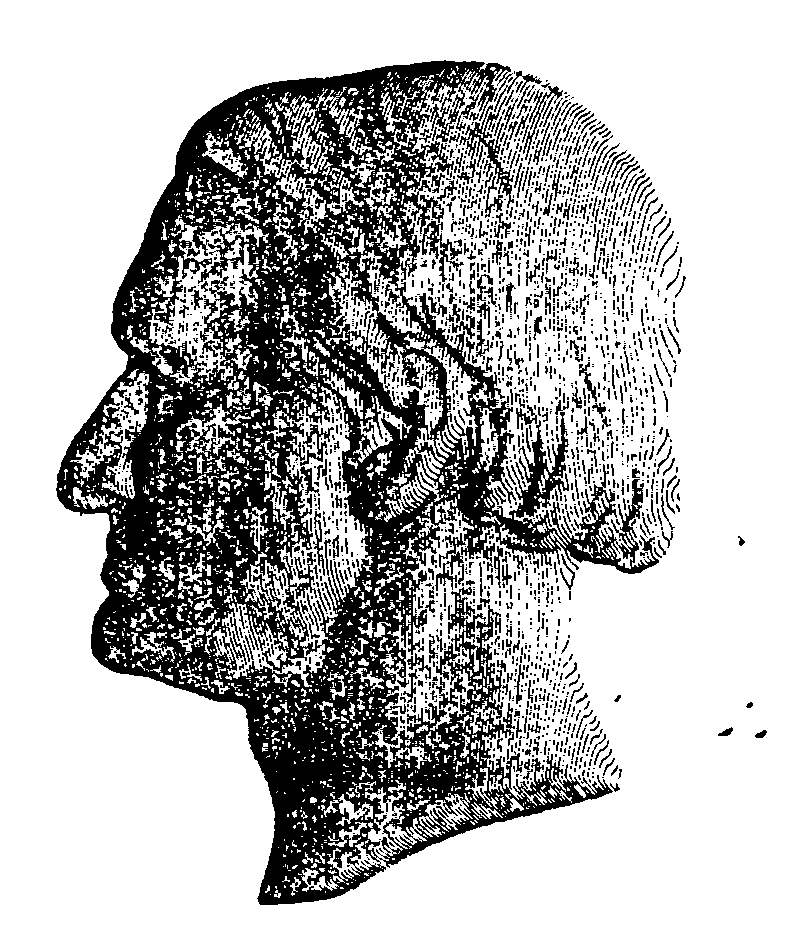
\includegraphics[height=2.2in]{figures/gauss_portrait_native004.png}\par
\vspace{.35in}
{\normalsize HERAUSGEGEBEN\par}
\medskip
{\small VON DER\par}
\medskip
{\normalsize KÖNIGLICHEN GESELLSCHAFT DER WISSENSCHAFTEN\par}
\medskip
{\small ZU\par}
\medskip
{\Large GÖTTINGEN\par}
\medskip
{\large 1867.\par}
\end{center}
\clearpage
\thispagestyle{empty}\SourceLeaf{5}
\pdfbookmark[0]{Theoria attractionis. Titulus}{attractionis-title}
\begin{center}
\vspace*{.45in}
{\large THEORIA ATTRACTIONIS\par}
\bigskip
{\Large CORPORUM SPHAEROIDICORUM\par}
\bigskip
{\large ELLIPTICORUM HOMOGENEORUM\par}
\bigskip
{\normalsize METHODO NOVA TRACTATA\par}
\vspace{.5in}
{\small AUCTORE\par}
\vspace{.5in}
{\large CAROLO FRIDERICO GAUSS\par}
\vspace{.55in}
{\small SOCIETATI REGIAE SCIENTIARUM TRADITA XVIII. MART. MDCCCXIII.\par}
\vfill
\rule{.8\textwidth}{.3pt}\par
\medskip
{\small Commentationes societatis regiae scientiarum Gottingensis recentiores. Vol.~\textsc{ii}\par}
\smallskip
Gottingae \textsc{mdcccxiii}.\par
\medskip
\rule{.8\textwidth}{.3pt}\par
\end{center}
\clearpage
